\section{System model and simulations}
This section thoroughly covers the models and simulations of the two subsystems that constitute the mechatronical system:
the mobile platform and the arm which is attached to the platform.
The software used in this project is covered in section~\ref{sec:implementation}.

\subsection{Model}

The system is modeled in two parts: the moving base and the\ldots
% TODO: describe the moving base, and the attachment, whatever it ends up being.
% Include physical models.


% Describe the states of the system.
We argue for the following five states of the system:
\begin{inline-enum}
\item waiting for a command;
\item moving to a destination;
\item following a navigation-line;
\item picking an object up; and
\item dropping an object off.
\end{inline-enum}
The relation between these five states are visually described in the state machine of Fig~\ref{fig:state_machine}.
\begin{figure*}[ht]
  \centering
  \begin{tikzpicture}
    \node[state, initial, accepting] (wait) {waiting for \\ command};
    \node[state, right of=wait] (move) {moving to \\ destination};
    \node[state, below of=move] (follow) {following \\ line};
    \node[state, right of=follow] (pickup) {picking \\ up object};
    \node[state, left of=follow] (dropoff) {dropping \\ off object};

    \path[->] (wait) edge node{Arrowhead \\ signal} (move)
    (move) edge[sloped] node{line detected \\} (follow)
    (follow) edge[sloped] node{station detection \\ (system w/o object)} (pickup)
    (follow) edge[sloped] node{station detection \\ (system w/ object)} (dropoff)
    (pickup) edge[sloped] node{object picked up \\} (move)
    (dropoff) edge[sloped] node{object dropped \\} (wait)
    ;
  \end{tikzpicture}
  \caption{High-level state machine of the system.}
  \label{fig:state_machine}
\end{figure*}

\subsubsection{Motor}
\begin{description}
\item[PID contoller for the LEGO EV3 motor]
The transfer function of the LEGO EV3 motor is assumed as eq.~\eqref{eq1}.This equation is called as second order transfer function. The input refers to the input power and the output refers to to wheel rotation in degrees.

\begin{equation}\label{eq1}
    G(s)=\frac{Y(s)}{U(s)}=\frac{W_n^2}{s^2+2\xi W_n s + W_n^2}
\end{equation}
where $W_n$ is the natural frequency and $\xi$ is the damping ratio.  These constants are given as:

\begin{equation}
\begin{split}
     W_n & = 14.2 \\
    \xi & = 0.92
\end{split}
\end{equation}
Then equation \ref{eq1} becomes :
\begin{equation}
    G(s)=\frac{201.9}{s^2+26.17s+201.9}
\end{equation}
The PID controller in the Laplace transform is described as
    \begin{equation}
    C(s)= K_P+K_I \frac{1}{s}+K_Ds= \frac{K_Ps+K_I+K_Ds^2}{s}
\end{equation}
where $K_p$,$K_I$ and $K_D$ is the proportional, integral and derivative terms respectively.
\item[Discretization of PID controller]
The PID-controller was discretized by zero order hold method. The ZOH method give a perfect match between continuous and discrete time domain. This method can also be used for system with input delays, output delays or transport delays and provides an exact discretization.
The eq. (\ref{eq5}) describes how to transform from s-domain to z-domain using Zero order hold method
\begin{equation} \label{eq5}
    C(z)=(1-z^{-1}) Z(\frac{C(s)}{s})
\end{equation}
where C(s) is the controller and Z is the Z-transform
\begin{equation}
    C(z)=(\frac{z-1}{z})Z(\frac{k_Ps+k_I+k_Ds^2}{s} \Big/ s)
    \label{eq7}
\end{equation}
By looking at the z-transform table, the eq.~\eqref{eq7} yields to
\begin{equation}
    C(z)=\frac{z-1}{z}\bigg( k_p \frac{1}{1-z^{-1}}+k_I \frac{T z^{-1}}{(1-z^{-1})^2}+k_D\bigg)
\end{equation}
And finally the PID controller in discrete time domain is presented as
\begin{equation}
    C(z)= k_P + k_I \frac{1}{z-1} + k_D \frac{z-1}{z}
\end{equation}

\item[Motor simulation]
The PID parameters were chosen to get low settling time, low overshoot and fast response to disturbances for the system. The best parameters for the system resulted in
\begin{equation}
    \begin{split}
        K_P & = 1.35 \\
        K_I & = 6 \\
        K_D & = 0.08 \\
    \end{split}
\end{equation}
The simulation is made in discrete time domain with a sampling frequency 10 Hz.
\begin{figure}[ht]
    \centering
    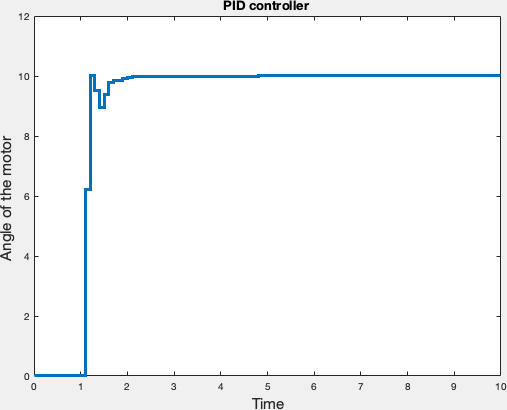
\includegraphics[width=0.4\textwidth]{sections/assets/pid_motor.png}
    \caption{PID controller for the LEGO EV3 motor to rotate 10 degrees}
    \label{fig1}
\end{figure}
\end{description}
\subsubsection{Trajectory planning}
A point to point trajectory is described as a path from $q_{init}$ to $q_{final}$. A trajectory is a function of time such that $q(t_0) = q_{init}$ and $q(t_f) = q_{final}$. The difference between $t_0$ and $t_f$ represents the total elapsed time to execute the trajectory. The velocity and the acceleration can be computed by differentiation since the trajectory is depending of time.
At the time $t_0$ the joint variable satisfies

\begin{equation} \label{eq10}
\begin{split}
     q(t_0) & = q_0 \\
    \dot{q}(t_0) & = v_0
\end{split}
\end{equation}
And at the $t_f$ the desired joint variable will be
\begin{equation} \label{eq11}
\begin{split}
     q(t_f) & = q_f \\
    \dot{q}(t_f) & = v_f
\end{split}
\end{equation}

The trajectory between two configurations and the initial and final velocity is known. One way to solve this task is to solve it by polynomial function of t. Since there are four unknown constraints, it is required to use a polynomial function with four independent coefficient. Hence a cubic trajectory is considered
\begin{equation} \label{eq12}
    q(t) = a_0 + a_1t + a_2t^2 + a_3t^3
\end{equation}
Then the velocity of the cubic trajectory becomes
\begin{equation} \label{eq13}
    \dot{q}(t) = a_1 + 2a_2t+ 3 a_3t^2
\end{equation}
Combining eq.~\eqref{eq12} and ~\eqref{eq13} with eq.~\eqref{eq10} and \ref{eq11} returns four equations with four unknowns
\begin{equation} \label{14}
    \begin{split}
        q_0 &= a_0 + a_1t_0 + a_2t_0^2 + a_3t_0^3 \\
        v_0 & = a_1 + 2a_2t+ 3 a_3t^2 \\
        q_f &= a_0 + a_1t_f + a_2t_f^2 + a_3t_f^3 \\
        v_f & = a_1 + 2a_2t_f+ 3 a_3t_f^2
    \end{split}
\end{equation}
Suppose taking $t_0 = 0$ and $t_f = 1$ second with velocity constraints as $v_0 = 0$ and $v_f = 0$. Then the eq. (\ref{14}) can be written in matrix form.
\begin{equation*}
    \begin{bmatrix}
1 & 0 & 0 & 0 \\
0 & 1 & 0 & 0 \\
 1 & 1& 1& 1 \\
0&1 &2 &3
\end{bmatrix} \begin{bmatrix}
a_0 \\
a_1 \\
a_2 \\
a_3
\end{bmatrix} = \begin{bmatrix}
q_0 \\
0\\
q_f \\
0
\end{bmatrix}
\end{equation*}
Then solving for the letter $a_i$ by linear algebra and this letters yields to
\begin{equation} \label{15}
    \begin{split}
        a_0 = q_0 \\
        a_1 = 0 \\
        a_2 = 3(q_f - q_0 ) \\
        a_3 = -2(q_f - q_0)
    \end{split}
\end{equation}
The eq. (\ref{eq12}) into eq. (\ref{15}) to get the cubic polynomial function. The required cubic polynomial function with the supposed constraints is therefore
\begin{equation}
    q_i(t) = q_0 + 3(q_f - q_0)t^2 - 2(q_f - q_0)t^3
\end{equation}
\begin{figure}[ht]
    \centering
    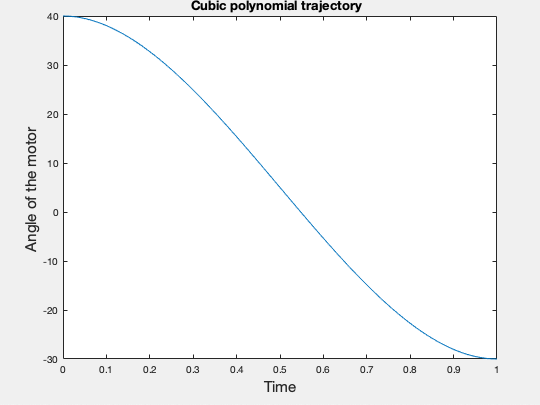
\includegraphics[width=0.4\textwidth]{sections/assets/cubic.png}
    \caption{Angle profile for cubic polynomial trajectory.}
    \label{fig2}
\end{figure}
Fig. (\ref{fig2}) shows the trajectory with $q_0 = 10^\circ$ and $q_f = -30^\circ$.


\subsubsection{Mobile platform}
\label{subsubsec:unicycle}
The model used in this case is the unicycle model, due to the differential steering.
This is because of the mobile platform has only two wheels/trucks and it is not able to apply any steering angle to its wheels.
The only way this robot can change orientation is by giving different velocity on each wheel-driving servo on left- and right- side.
With this feature it is also possible to change the orientation of the mobile platform without changing the position of the platform.
I.e. the robot is able to spin while the right-hand side wheels have the same velocity as the left-hand side wheels, in opposite direction.
\begin{figure}[h]
\centering
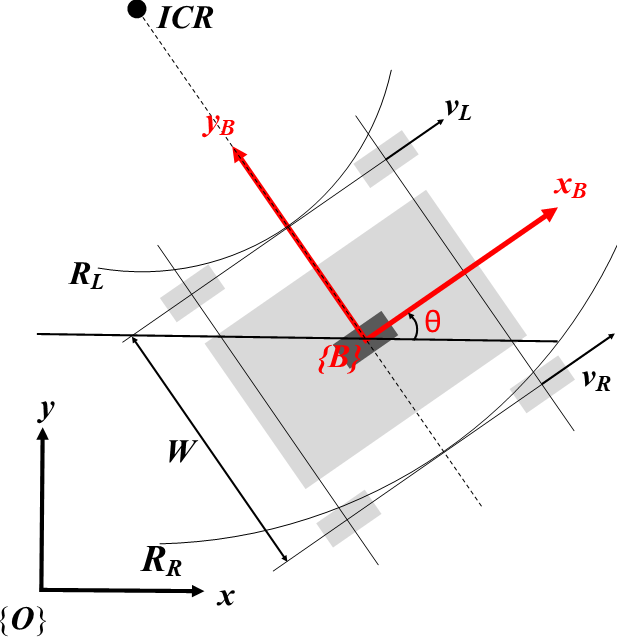
\includegraphics[width=0.4\textwidth]{sections/assets/car-unicycle.png}
\caption{Unicycle model of a car-like robot.
$v_L$ and $v_R$ represent the left- and right-hand side wheels' velocities respectively.
The robot follows a path around the instantaneous center of rotation (ICR) where $R_L$ and $R_R$ are the distances from left and right wheels to ICR respectively and $w$ is the distance between them.}
\label{fig:UnicycleModel}
\end{figure}

As shown in Fig.~\ref{fig:UnicycleModel} The robot follows a curved path with the instantaneous center of rotation at its center.
The left-hand side wheels have velocity $v_L$ and moves along an arc with radius $R_L$ during the time that right-hand side wheels moves along another arc with radius $R_R$ at the speed of $v_R$.
The turning rate of the body is
\begin{equation*}
\dot{\theta}= \frac{v_L}{R_L} = \frac{v_R}{R_R}
\end{equation*}
since $R_R = R_L + W$ the expression can be simplified as
\begin{equation}
\dot{\theta}= \frac{v_R - v_L}{W} = \frac{v_\Delta}{W}\label{eq:ThetaDot}
\end{equation}
the equations of motion for this model are
\begin{eqnarray}
\begin{aligned}
\dot{x} &= v\,cos(\theta)\\
\dot{y} &= v\,sin(\theta)\\
\dot{\theta} &= \omega = \frac{v_\Delta}{W}
\end{aligned}
\label{eq:MotionEq}
\end{eqnarray}
where the average velocity \parencite{Corke2011} is given by
\begin{equation}
v = \frac{v_R + v_L}{2}
\label{eq:av_velocity}
\end{equation}
Before the implementation, it is required to to find a discrete equivalent for the systems dynamics.
By being able to count the number of encoder ticks on each servo and some approximation it is possible to estimate the position of the robot.
In this approximative method we assume that the driven path in-between the two sampling points is a straight line. 
The length of the driven path for each wheel can be computed using the following formula:

\begin{equation}
    D = 2\,\pi\,r\,\frac{\Delta tick}{N}
\end{equation}\label{eq:encoder-formula}
Where $D$ is the length of the driven path, $r$ is the wheel radius, $\Delta tick$ is the number of recorded ticks during the two sampling points and $N$ is the number of ticks per revolution.
In our case the numeric values are:

\begin{eqnarray*}
    r =& 0.021\, [m]\\
    N =& 360\, [\frac{tick}{2\,\pi}]
\end{eqnarray*}
In this report we will use the notations $D_r$ and $D_l$ for the length of the driven path for the right- and left- hand side wheels respectively. 
$D_c$ is the notation we use for the length of the driven path for the body and is similar to Eq.~\eqref{eq:av_velocity}:

\begin{equation}
    D_c = \frac{D_r + D_l}{2}
\end{equation}
The discretized equations of motion is given by:

\begin{eqnarray}
\begin{aligned}
    x(k+1) =& x(k) + D_c(k)\,cos(\theta(k))\\
    y(k+1) =& y(k) + D_c(k)\,sin(\theta(k))\\
    \theta(k+1) =& \theta(k) + \frac{D_r(k)-D_l(k)}{W}
\end{aligned}
\end{eqnarray}\label{eq:Disc_EOM}
Where $W$ is the width of the robot, i.e. the distance between the two wheels.
The limitation of this approximative method is the sampling rate relative the average velocity of the body.
The arc shaped driven path is being approximated by dividing the curve in to several points and recreate a polygonal path using line segments to connect this points together. 
E.g. if the average velocity is very high and the sampling rate is very low, the straight line will not be a good approximation for the driven arc shaped path.
To make this approximation more accurate it is required to divide the driven path in to more points.
This accuracy can be improved by having higher sampling rate or lower average velocity.

\subsubsection{Arm}

\subsection{Simulation}
% Simulte the models from the previous section and show that it will work.
% Motivate regulation approach.
\subsubsection{Mobile platform}
A simulation profile is made to make sure of the unicycle mode in sub section ~\ref{subsubsec:unicycle} is the suitable model for this application.
The simulation is made in discrete time domain with the sampling frequency of $10$~Hz.
This is done in the described way due to the robot is going to operate in discrete time.
The sampling frequency is assumed to be low and that is because the designed controllers are going to be able to work fine for higher samplings frequencies but that is not guaranteed for vise-versa.
As the unicycle model describes the systems dynamics.
The position of the robot $(x, y, \theta)$ is dependent on the two wheel velocities. Which in turn has dependencies to the average velocity $V$ and the angular velocity $\omega$. These relations are presented in Eq.~\eqref{eq:ThetaDot} -- Eq.~\eqref{eq:av_velocity}.
\begin{figure*}[h]
\centering
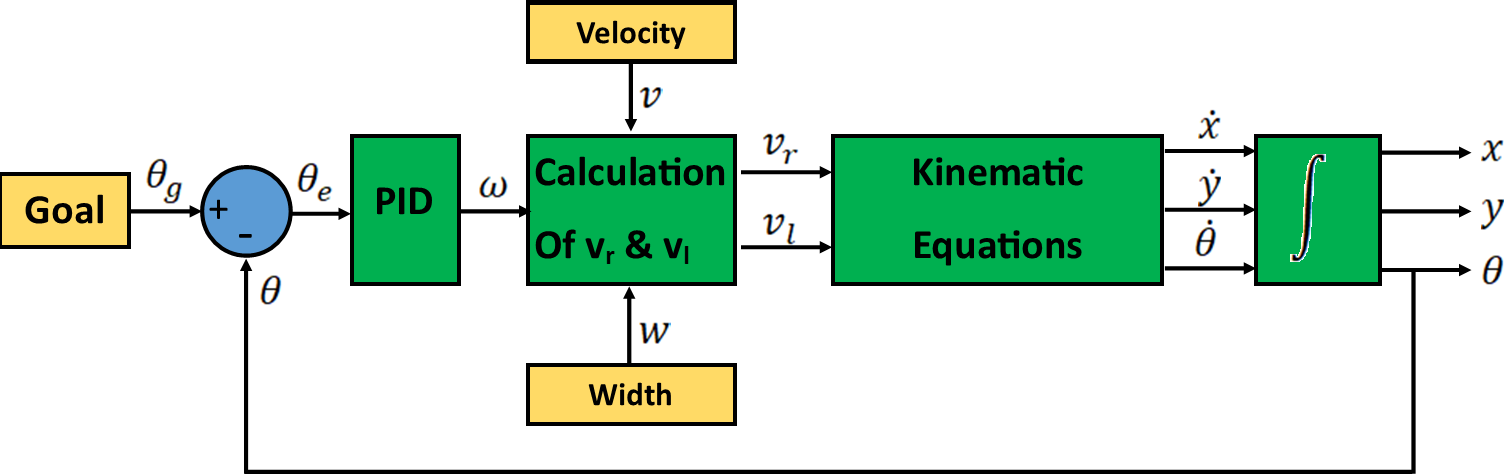
\includegraphics[width=\textwidth]{sections/assets/omegaCtrlr.png}
\caption{Overview of the systems block diagram where the angular velocity $\omega$ is controlled by a PID controller.}
\label{fig:overview}
\end{figure*}

A pole placement analyze is required for the design of a PID controller.
This analyze is done in continues time domain, due to its simplicity.
As mentioned in Eq.~\eqref{eq:MotionEq}
\begin{equation}
\dot{\theta} = \omega
\label{eq:omega}
\end{equation}
By taking the Laplace transform of Eq.~\eqref{eq:omega} gives:
\begin{equation}
s\cdot \Theta(s)= \Omega(s)
\end{equation}
Where $G(s)$ is the transfer function
\begin{equation}
\therefore G(s)=\frac{\Omega(s)}{s\cdot\Theta(s)} = 1
\end{equation}
However it is the angular position $\theta$ which is relevant in this case.
So it is required to implement an integrator in the feedback to make the angular position controllable.
\tikzset{
    block/.style = {draw, rectangle,
    minimum height=1cm,
    minimum width=2cm},
    input/.style = {coordinate,node distance=1cm},
    output/.style = {coordinate,node distance=2cm},
    arrow/.style={draw, -latex,node distance=2cm},
    pinstyle/.style = {pin edge={latex-, black,node distance=2cm}},
    sum/.style = {draw, circle, node distance=1cm}
}
\begin{figure}[h]
    \begin{center}
        \begin{tikzpicture}[auto, node distance=2.5cm,>=latex']
        \node [input, name=input] {};
        \node [sum, right of=input] (sum) {};
        \node [block, right of=sum] (controller) {$PID$};
        \node [block, right of=controller] (plant) {$G(s)$};
        \node [output, right of=plant] (output) {};
        \node [block, below of=plant] (feedback) {$\frac{1}{s}$};
        \draw [draw,->] (input) -- node {$U(s)$} (sum);
        \draw [->] (sum) -- node {} (controller);
        \draw [->] (controller) -- node {} (plant);
        \draw [->] (plant) -- node [name=y] {$Y(s)$}(output);
        \draw [->] (y) |- node [above,pos=0.79] {} (feedback) ;
        \draw [->] (feedback) -| node[pos=0.99] {$-$}
        node [near end] {} (sum);
        \end{tikzpicture}
    \end{center}
    \caption{Closed loop system with a integrator in the feedback.}\label{fig:closedloop}
\end{figure}

In this case the closed loop transfer function will be as shown in Eq.~\eqref{eq:closedloop}
\begin{equation}
G_{c}(s) = \frac{PID}{s + PID}
\label{eq:closedloop}
\end{equation}
As the closed loop transfer function of the system is describing a first order system, it is possible to use a P-controller.
I.e. the controller only has a proportional gain and doesn't require a integrative or derivative elements.
So the final closed loop transfer function will be
\begin{equation}
G_{c}(s) = \frac{K_p}{s + K_p}
\label{eq:kp}
\end{equation}

This system will have a pole at $-K_p$.
Any positive proportional gain will results in a stable pole and which in turn leads to a stable system.
\begin{figure*}[ht]
\centering
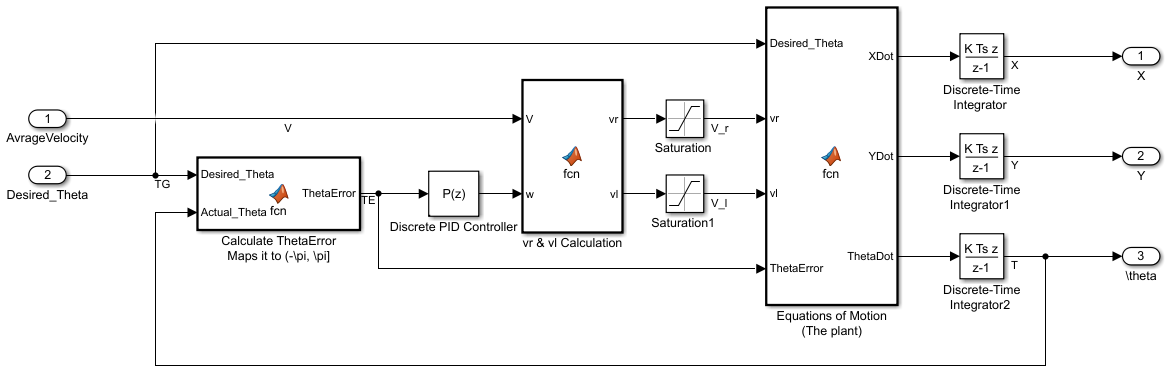
\includegraphics[width=\textwidth]{sections/assets/Theta_PID.PNG}
\caption{The complete control block for the angular position in discrete time domain.}
\label{fig:PID1}
\end{figure*}

It is required to make sure that $\theta$ error, $\theta_e$ is in $(-\pi,\pi]$ span. Due to the $\theta = \theta \pm 2 \cdot n \cdot \pi$, it is possible for the error be in out of this span.
By using a function called arctan2 or atan2 in many programming languages it is possible to accomplish this challenge.
This function often has two input argument (y,x).
By defining
\begin{equation}
\theta = \text{atan2}(\sin(\theta),\, \cos(\theta))
\end{equation}
$\theta$ will always be in $(-\pi,\pi]$ span.

Due to the physical limits the servos have, two saturation blocks are required.
These blocks are shown in Fig.~\ref{fig:PID1} and the assumption for their limits are $(-10,10)$~[cm/s].
This assumption is done to make the simulation more alike the real application.
\begin{figure}[ht]
\centering
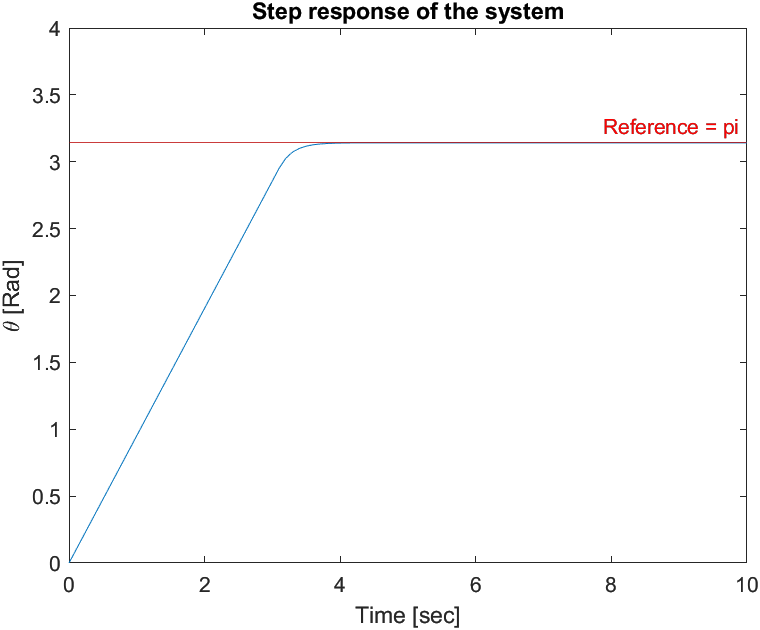
\includegraphics[width=0.4\textwidth]{sections/assets/Theta_pi_stepresponse.png}
\caption{The step response for $\theta$ where the proportional gain $K_p = 4$ and the reference value is $\pi$.}
\label{fig:Theta_Step}
\end{figure}

The result of the simulation, the step response for the angular position control system is presented in Fig.~\ref{fig:Theta_Step}.
As it shown this is a stable system, it has no steady state error, no oscillation and relative fast rise-time.

In this part of the mobile platforms movement it is important to be able to control the spacial position $(x, y)$.
As shown in the kinematic equations Eq.~\eqref{eq:MotionEq} the positions are dependent on both the angular velocity $\omega$ and the average velocity $v$.
A design of a controller for the average velocity is required to make it possible to control the spacial position.
Take note of the two input \texttt{AverageVelocity}, \texttt{Desired\_Theta} and the two output \texttt{X}, \texttt{Y} in Fig.~\ref{fig:PID1}.

By redefining the spatial error from a Cartesian coordinate system to a polar coordinate system it is possible to design a controller for average velocity.
In this case the error will be defined as following:
\begin{eqnarray}
\begin{aligned}
\Delta x &= Desired\_X - X\\
\Delta y &= Desired\_Y - Y\\
Distance &= \sqrt{\Delta x^2 + \Delta y^2}\\
Desired\_\theta &= \text{atan2}(\Delta y, \Delta x)
\end{aligned}
\label{eq:cart2polar}
\end{eqnarray}

Now by defining the distance as an error to a PID controller for the average velocity, it makes it possible for the mobile platform to stop at the desired position.
In this case a P controller, a controller which has only a proportional gain, is enough.
\begin{figure*}[h]
\centering
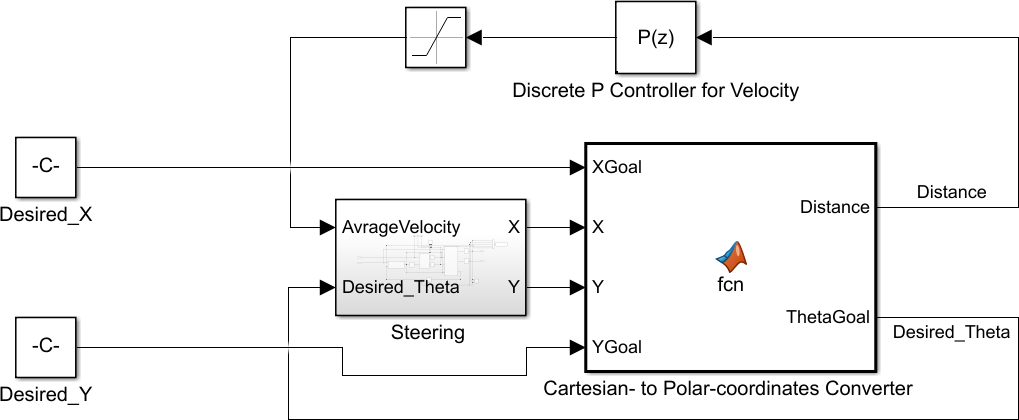
\includegraphics[width=\textwidth]{sections/assets/V_PID.PNG}
\caption{Overview of the complete systems block diagram for the spatial position control. Fig.~\ref{fig:PID1} is an overview of the ``Steering'' block and Eq.~\eqref{eq:cart2polar} is the mathematical definition for the block function ``Cartesian- to Polar-coordinates Converter''.}
\label{fig:V_PID}
\end{figure*}

Here comes some of the results for the spacial position control simulation. In this case the desired position is $(100, 100)$, the proportional gain for the angular velocity controller is $K_p = 4$ and the proportional gain for the average velocity controller is $K_p = 5$. If you are interested to see more plots, you can go to the Git-repository under \texttt{simulation/Diff\_Drive/README.txt} and you will find out how to generate more relative plots for this system.

\begin{figure}[h]
\centering
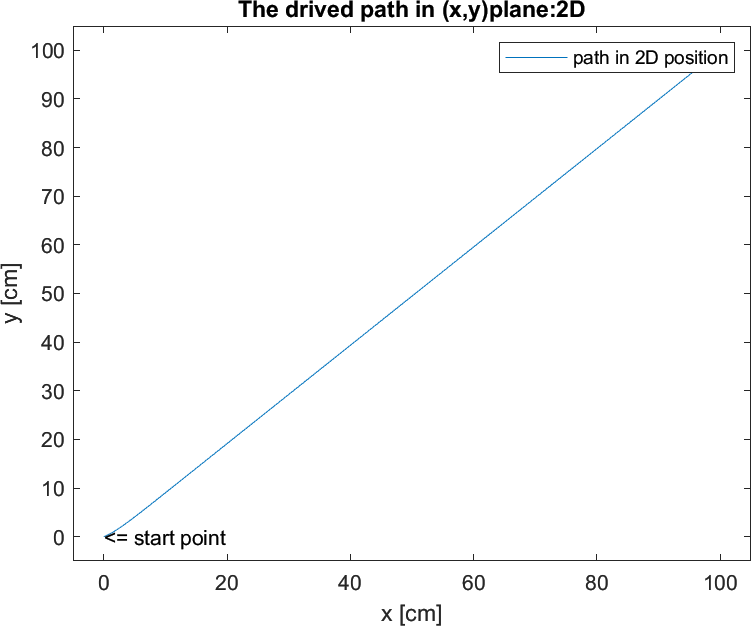
\includegraphics[width=0.4\textwidth]{sections/assets/traj.png}
\caption{The driven trajectory.}
\end{figure}

\begin{figure}[h]
\centering
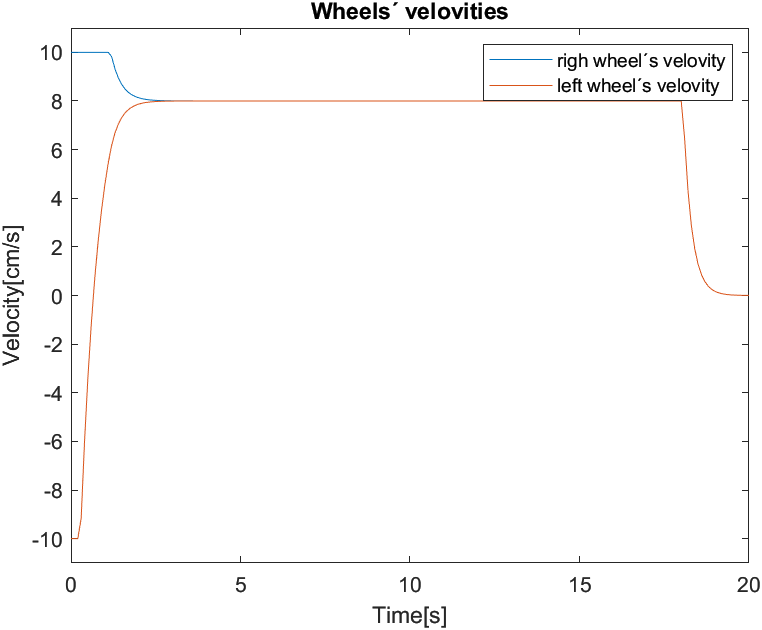
\includegraphics[width=0.4\textwidth]{sections/assets/WV.png}
\caption{The wheels' velocities during the drive time.}
\end{figure}

\subsubsection{Arm}

\subsection{Hardware}
% Explain the raspberry pi and it's attachments, the motors, and all the lego
